\documentclass[]{article}
\usepackage{lmodern}
\usepackage{amssymb,amsmath}
\usepackage{ifxetex,ifluatex}
\usepackage{fixltx2e} % provides \textsubscript
\ifnum 0\ifxetex 1\fi\ifluatex 1\fi=0 % if pdftex
  \usepackage[T1]{fontenc}
  \usepackage[utf8]{inputenc}
\else % if luatex or xelatex
  \ifxetex
    \usepackage{mathspec}
  \else
    \usepackage{fontspec}
  \fi
  \defaultfontfeatures{Ligatures=TeX,Scale=MatchLowercase}
\fi
% use upquote if available, for straight quotes in verbatim environments
\IfFileExists{upquote.sty}{\usepackage{upquote}}{}
% use microtype if available
\IfFileExists{microtype.sty}{%
\usepackage[]{microtype}
\UseMicrotypeSet[protrusion]{basicmath} % disable protrusion for tt fonts
}{}
\PassOptionsToPackage{hyphens}{url} % url is loaded by hyperref
\usepackage[unicode=true]{hyperref}
\hypersetup{
            pdfborder={0 0 0},
            breaklinks=true}
\urlstyle{same}  % don't use monospace font for urls
\usepackage[margin=1in]{geometry}
\usepackage{graphicx,grffile}
\makeatletter
\def\maxwidth{\ifdim\Gin@nat@width>\linewidth\linewidth\else\Gin@nat@width\fi}
\def\maxheight{\ifdim\Gin@nat@height>\textheight\textheight\else\Gin@nat@height\fi}
\makeatother
% Scale images if necessary, so that they will not overflow the page
% margins by default, and it is still possible to overwrite the defaults
% using explicit options in \includegraphics[width, height, ...]{}
\setkeys{Gin}{width=\maxwidth,height=\maxheight,keepaspectratio}
\IfFileExists{parskip.sty}{%
\usepackage{parskip}
}{% else
\setlength{\parindent}{0pt}
\setlength{\parskip}{6pt plus 2pt minus 1pt}
}
\setlength{\emergencystretch}{3em}  % prevent overfull lines
\providecommand{\tightlist}{%
  \setlength{\itemsep}{0pt}\setlength{\parskip}{0pt}}
\setcounter{secnumdepth}{0}
% Redefines (sub)paragraphs to behave more like sections
\ifx\paragraph\undefined\else
\let\oldparagraph\paragraph
\renewcommand{\paragraph}[1]{\oldparagraph{#1}\mbox{}}
\fi
\ifx\subparagraph\undefined\else
\let\oldsubparagraph\subparagraph
\renewcommand{\subparagraph}[1]{\oldsubparagraph{#1}\mbox{}}
\fi

% set default figure placement to htbp
\makeatletter
\def\fps@figure{htbp}
\makeatother

\usepackage{etoolbox}
\makeatletter
\providecommand{\subtitle}[1]{% add subtitle to \maketitle
  \apptocmd{\@title}{\par {\large #1 \par}}{}{}
}
\makeatother
\usepackage{setspace}\doublespacing
\usepackage{lineno}\linenumbers
% https://github.com/rstudio/rmarkdown/issues/337
\let\rmarkdownfootnote\footnote%
\def\footnote{\protect\rmarkdownfootnote}

% https://github.com/rstudio/rmarkdown/pull/252
\usepackage{titling}
\setlength{\droptitle}{-2em}

\pretitle{\vspace{\droptitle}\centering\huge}
\posttitle{\par}

\preauthor{\centering\large\emph}
\postauthor{\par}

\predate{\centering\large\emph}
\postdate{\par}

\date{}

\begin{document}

\section{Pagel's Lambda Estimates are Often
Inaccurate}\label{pagels-lambda-estimates-are-often-inaccurate}

\hfill\break

\textbf{Keywords}: Pagel's lambda, phylogenetic signal \hfill\break

\textbf{Short Title}: Inaccuracies in Pagel's Lambda \hfill\break

\section{Abstract}\label{abstract}

\{conclusion holds: interpreting the regression is not appreciably
different (in terms of slopes and f values)\}

\newpage

\section{Introduction}\label{introduction}

Investigating macroevolutionary patterns requires a phylogenetic
approach as species are non-independent by nature of their shared
ancestry. Since the first appropriate method was introduced by
Felsenstein (phylogenetic independent contrasts; Felsenstein (1985)),
dozens of other methods have been developed and applied to increasingly
complex questions in macroevolutionary biology (e.g. Grafen (1989);
Harvey and Pagel (1991); Rohlf (2001); ({\textbf{???}})). A particularly
useful measure in this field is phylogenetic signal, a quantification of
a trait's correspondence with the clade's phylogenic history.
Understanding the degree of phylogenetic signal present in a dataset is
paramount and identifies the mode under which a trait has evolved; high
measures of phylogenetic signal indicate a Brownian motion process,
whereas lower levels of phylogenetic signal indicate natural selection
or some other evolutionary force has influenced the traits evolutionary
history. \hfill\break

Several approaches to quantify phylogenetic signal exist. For continuous
data, the most common parameters used in the literature include Pagel's
lambda ({\textbf{???}}) and Blomberg's kappa ({\textbf{???}}). Pagel's
lambda has the advantage of being nested in the likelihood framework and
thus has also been utilized to simultaneously estimate and account for
phylogenetic signal while doing phylogenetic regressions or ANOVAs. At
the development of these estimation methods, clear recommendations on
the use and interpretation of this parameter were made based on data
simulations and error evaluations (Revell 2010). However, the accuracy
of the lambda estiamtion methods have not been fully evaluated, and
consequently many studies have substantially misused these methods.
\hfill\break

An earlier study ({\textbf{???}}), breifly addressed this topic by
showing how uninformative smaller phylogenies are when estimating
various evolutionary parameters, such as Pagel's lambda. However, it
remains unknown the degree to which lambda estimates accurately
represent degree of phylogenetic signal, and thus we fully explicate the
extent to which Pagel's lambda estimation methods can and have been
misused in recent macroevolutionary studies. Here we take a
comprehensive approach to demonstrate the scenarios under which
estimated Pagel's lambdas accurately reflect known lambdas. We then
demonstrate the effect of these, at times, dubious estimation methods on
significance testing when used in a PGLS framework. Finally, we perform
a meta-analysis of research published in 2019 employing Pagel's lambda
estimation methods to demonstrate the uses and misuses of this method in
the literature. This investigation provides evidence for the
circumstances under which estimating Pagel's lambda can be informative,
and which interpretations or uses are misleading with the hope of moving
the field towards more appropriate employment of phylogenetic
comparative methods.

\section{Methods and Results}\label{methods-and-results}

\subsection{\texorpdfstring{\emph{Simulated
trait}}{Simulated trait}}\label{simulated-trait}

To assess the accuracy of Pagel's lambda estimations, we simulated
pure-birth phylogenies of variable size, ranging in tip number from 32
to 1024. We then scaled the simulated phylogenies by lambda values
ranging from 0 to 1 (0.05 intervals; 50 trees per lambda value per tree
size) with which we generated trait data with known lambdas by
simulating a continuous variable on each scaled phylogeny under Brownian
motion. We then estimated lambda values from these data using
phylogenetic generalized least squares (PGLS) to compare against the
known lambda values. \hfill\break

To visualize the accuracy of the lambda estimation methods, we first
plotted known lambdas (input lambdas) against the estimated lambdas
(Figure 1). This plot demonstrates the rampant inaccuracy of estimating
lambdas on phylogenies with fewer than 200 tips, as the spread of data
in the upper panels in Figure 1 is remarkably wide. We also see that the
widest spread of estimated lambdas is observed near the center of each
plot corresponding to intermediate values of known lambda. Lastly, we
see a slight tendency for the PGLS estimation methods to underestimate
lambda, especially for known lambda values below 0.5 as can be seen by
the numerous data points along the x axis for the smaller phylogenies
analyzed (n tips \textless{} 200). \hfill\break

{[}insert Figure 1 here{]}

\subsection{\texorpdfstring{\emph{Simulated ANOVA and
Regressions}}{Simulated ANOVA and Regressions}}\label{simulated-anova-and-regressions}

To measure the statistical performance of PGLS lambda estimation methods
when applied to ANOVA and regression analyses, we used the above
generated data (independent variables) to simulate a second set of trait
variables (depedendent variables) across the range of correlation
strengths (betas ranging from 0 to 1 at intervales of 0.25). We then
used PGLS to estimate phylogenetic signal of the dependent variable and
the slope coefficient for the regression between the dependent and
independent variables. We also calculated F- and p-values from the
regression analyses. Finally, we again fit the dependent variable to the
independent variable while holding the lambda value at 0 to approximate
an ordinary least squares (OLS) apprach. \hfill\break

We compared the estimated slope coefficients across variable input beta
values to assess the ability of PGLS to identify significant
correlations (Figure 2). All distribution groups center around the 1:1
relationship between input beta values and estimated slopes. However the
variance around that mean is substantial, with estimates ranging from
approximately -2 to 4 in datasets with 32 taxa and a known relationship
of (beta = 1). This variance of the estimated slopes only becomes
reasonable when phylogenies have over 200 tips, similarly to what we saw
in the first simulation analysis in this study. \hfill\break

{[}insert Figure 2 here{]} \hfill\break 

Surprisingly, the estimated lambda values of the dependent variable do
not correspond with input lambda values that characterize the
independent variable (Figure S1). This disconnect then resulted in no
appreciable difference of slope estimates across input lambda values
(Figure S2), nor do we see substantial differences in slope estimates
between the PGLS and OLS analyses (results not shown). Thus, we show
that phylogenetic signal present in one variable does not translate to
phylogenetic signal in a second, even highly correlated, dependent
variable. \hfill\break

Scaling and trait generation procedures for all simulation methods were
repeated with symmetrical and ladder phylogenies of variable size.
Results generated using these variable phylogeny shapes were consistent
with the pure-birth phylogeny results presented above and can be found
in the Supplemental Materials. All analyses were performed in R v3.6.0
({\textbf{???}}) using the packages \texttt{geiger} ({\textbf{???}}) and
\texttt{caper} ({\textbf{???}}), and the corresponding scripts can be
found in the Supplemental Materials.

\subsection{\texorpdfstring{\emph{Meta-Analysis of Empirical
Results}}{Meta-Analysis of Empirical Results}}\label{meta-analysis-of-empirical-results}

To understand the extent of this problematic estimation method in
application, we performed a meta-analysis of studies published in 2019
that cited Pagel's 1997 manuscript ({\textbf{???}}). The list of
manuscripts was compiled through Google Scholar on Jan 23, 2020 and
totaled 341 manuscripts. For each study, we extracted any published
lambda estimates, along with the size of the phylogeny used in the
analysis. We also noted whether authors reported confidence intervals,
significance tests assessing difference of the lambda estimate from 0 or
1, and whether authors interpreted biological meaning from the magnitude
of the estimated lambda. For studies that reported more than one lambda
estimate, we also noted if the authors compared the lambdas against one
another, and whether that was accompanied with an appropriate
statistical test between the estimated lambda values. \hfill\break

We found 182 manuscripts from 2019 that estimated and reported Pagel's
lambda values using PGLS methods. These papers averaged 8.527 lambda
values, ranging from a single lambda estimate up to 71 estimated
lambdas. Almost exactly half of the published lambda estimates were
either below 0.05 (25.32\%) or above 0.9 (24.74\%; Figure 3). 73.32\% of
the published lambdas were estimated using phylogenies with fewer than
200 tips, and 348 lambda estimates (8.57\% of all published estimates)
came from phylogenies with fewer than 30 tips. \hfill\break

{[}insert Figure 3 here{]} \hfill\break

Many of the reviewed manuscripts liberally interpreted the magnitude of
the estimate lambda, using phrases such as ``strong'' or ``weak''
phylogentic signal when statistically, all that was clear was a
difference between the estimated lambda and 0 or 1 respectively. We
estimated that about 20.49\% of the manuscripts revealed some sort of
biological interpretation of the magnitude of estimated phylogenetic
signal that overreached the statistical findings. We also identified
seven manuscripts as having inappropriately interpreted differences in
lambda values, indicating that some traits had stronger or weaker signal
than other traits without the appropriate statistical tests.
\hfill\break

As is evidenced by macroevolutionary papers published in 2019 papers,
Pagel's lambda estimation methods are often misused and
over-interpretted. Despite the urging of Boettiger and colleagues to
publish confidence intervals with all lambda parameter estimates, only
18\% of papers published in 2019 do so.

\section{Discussion}\label{discussion}

{[}This part is obviously not written yet{]} \hfill\break

General conclusions :Using the estimated lambda values from pgls are not
useful. The questions of whether or not signal exists is appropriate,
but inferring more from lambda \emph{magnitude} is inappropriate.
\hfill\break

More discussion paragraphs

\newpage

\section{References}\label{references}

\setlength{\parindent}{-0.25in} \setlength{\leftskip}{0.25in}
\setlength{\parskip}{8pt} \noindent

\hypertarget{refs}{}
\hypertarget{ref-Felsenstein1985}{}
Felsenstein, J. 1985. Phylogenies and the comparative method. American
Naturalist 125:1--15.

\hypertarget{ref-Grafen1989}{}
Grafen, A. 1989. The phylogenetic regression. Philosophical Transactions
of the Royal Society of London B, Biological Sciences 326:119--157.

\hypertarget{ref-HarveyPagel1991}{}
Harvey, P. H., and M. D. Pagel. 1991. The comparative method in
evolutionary biology. Oxford University Press, Oxford.

\hypertarget{ref-Revell2010}{}
Revell, L. J. 2010. Phylogenetic signal and linear regression on species
data. Methods in Ecology and Evolution 1:319--329.

\hypertarget{ref-Rohlf2001}{}
Rohlf, F. J. 2001. Comparative methods for the analysis of continuous
variables: Geometric interpretations. Evolution 55:2143--2160.

\newpage

\section{Figure Legends}\label{figure-legends}

\textbf{Figure 1}. Accuracy of Pagel's lambda estimations across known
lambda inputs on various tree sizes. As trees increase in size, the
estimates more closely resemble the input lambdas, however considerable
and concerning variation is apparent in trees smaller than those with
200 tips. \hfill\break

\textbf{Figure 2}. Estimated ANOVA slopes under PGLS. Across tree sizes,
the mean estimated slope matches the input slope, and as trees increase
in size, the variance around this mean estimate decreases. However, for
trees with fewer than 200 tips, the error around the estimated slope is
considerable, where these analyses frequently estimate slopes in the
opposite direction of the known pattern. \hfill\break

\textbf{Figure 3}. Frequency of estimated lambda values published in
manuscripts in 2019. The majority of these values were close to 0 or 1,
and from phylogenies with fewer than 200 taxa.

\newpage

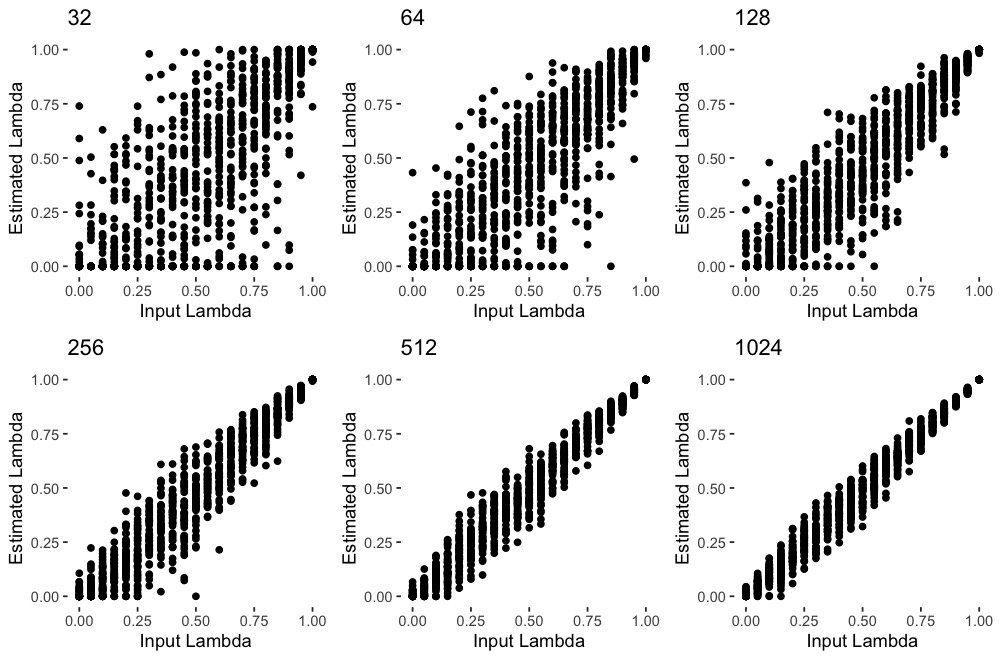
\includegraphics[width=0.95\linewidth]{Fig1}

\singlespacing \textbf{Figure 1}. Accuracy of Pagel's lambda estimations
across known lambda inputs on various tree sizes. As trees increase in
size, the estimates more closely resemble the input lambdas, however
considerable and concerning variation is apparent in trees smaller than
those with 200 tips. \hfill\break

\newpage

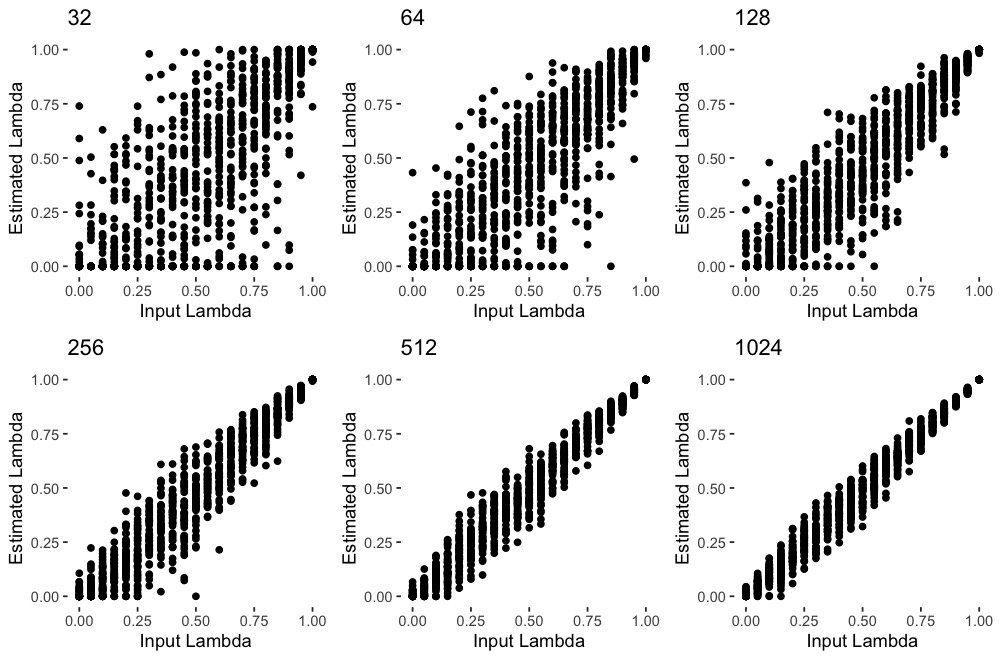
\includegraphics[width=0.95\linewidth]{Fig2}

\singlespacing \textbf{Figure 2}. Estimated ANOVA slopes under PGLS.
Across tree sizes, the mean estimated slope matches the input slope, and
as trees increase in size, the variance around this mean estimate
decreases. However, for trees with fewer than 200 tips, the error around
the estimated slope is considerable, where these analyses frequently
estimate slopes in the opposite direction of the known pattern.
\hfill\break

\newpage

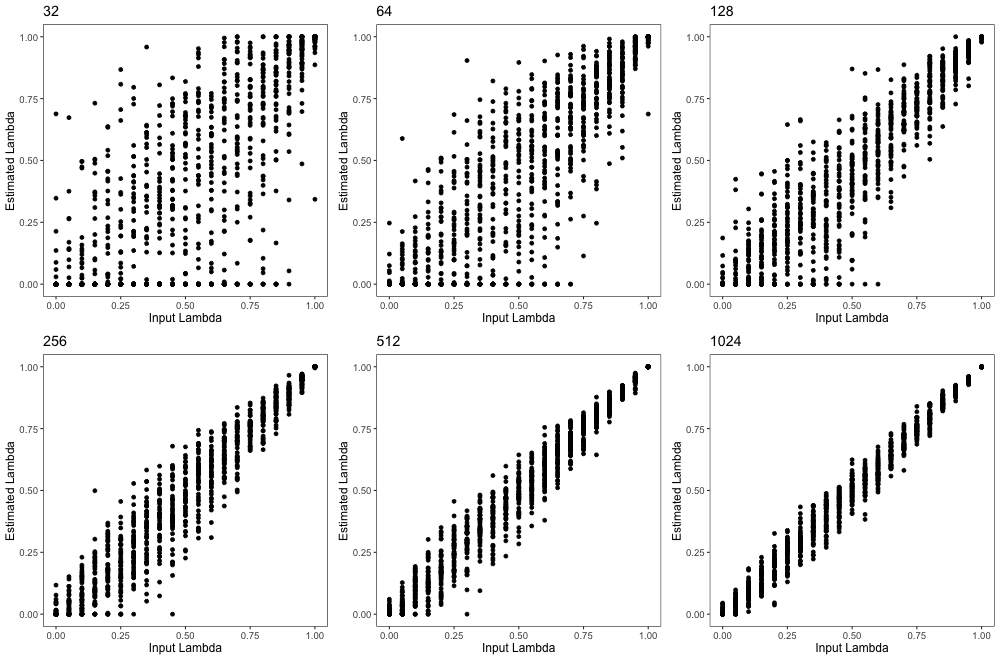
\includegraphics[width=0.95\linewidth]{Fig3}

\singlespacing \textbf{Figure 3}. Frequency of estimated lambda values
published in manuscripts in 2019. The majority of these values were
close to 0 or 1, and from phylogenies with fewer than 200 taxa.

\end{document}
